\section{StyleGAN Modulation / Demodulation, Attention is all you need}

    Πρόσφατες μέθοδοι εφαρμόζουν μηχανισμό σύγχρονης/ \enit{online}  ενσωμάτωσης των βαθιών χαρακτηριστικών  που παράγουν τα δίκτυα κωδικοποίησης \footnote{όπως και τα \enit{DeepSDF embedding} της εργασίας} στα βάρη του δικτύου.
    Με αυτό το σκεπτικό αντλήθηκαν πληροφορίες από δίκτυα που εφαρμόζουν διαμόρφωση και αποδιαμόρφωση του χαρακτηριστικών σκοπεύοντας την ομαλοποίηση των δικτύων και την προσθήκη στο επίπεδο γνώσης του \enit{style}/στιλ των δεδομένων. Αυτή η έννοια δεν αναφέρεται κυριολεκτικά αλλά αναφέρεται σε στατιστικές που έχουν τα δεδομένα και στην απόκτηση γνώσης μέσα από αυτές. 
    
    Αρχικά παρουσιάστηκε μια έρευνα πάνω στην προσαρμοστική κανονικοποίηση του δικτύου. Αυτή (\enit{Adaptive Instance Normalization} \cite{huang2017arbitrary}) στοχεύει το ίδιο το δεδομένο εισόδου και όχι με βάση τις ομάδες δεδομένων (\enit{batches}) εκπαίδευσης που περνούν από το δίκτυο μέχρι την επόμενη αναβάθμιση των βαρών. Το τελευταίο είναι κλασσική τακτική, που στην ορολογία των νευρωνικών δικτύων αναφέρεται ως \enit{Batch Normalization}. Αυτού του είδους η προσαρμοστική κανονικοποίηση δείγματος,  θεωρεί μη αποδοτική την χρήση \enit{Batch Normalization} καθώς κανονικοποιεί τα δεδομένα με βάση την στατιστική ενός πλήθους δειγμάτων, διαισθητικά ομαλοποιώντας όλο το \enit{batch} γύρω από ένα κεντρικό στυλ που φαίνεται από τις στατιστικές του χαρακτηριστικού. Στην περίπτωση των δικτύων ανακατασκευής που δέχονται ως είσοδο συντεταγμένες, και επομένως σχηματίζουν χαρακτηριστικά διανύσματα συντεταγμένων, κάθε δείγμα δεδομένων είναι σημαντικό ως προς τις στατιστικές του. Συνεπώς ο \enit{AdaIN} αλγόριθμος προσπαθεί να εφαρμόσει το στυλ της εισόδου στα δεδομένα που περνούν από το δίκτυο κάνοντας χρήση ανακλιμάκωσης του πίνακα χαρακτηριστικών (\enit{rescaling feature map}) με βάση ένα διάνυσμα στατιστικών της εισόδου υπολογίζεται (\enit{Style Vector}).

\par
    Πάνω σε αυτή την μέθοδο, η ήδη υπάρχουσα έρευνα \enit{StyleGAN} που προτείνει ένα παραγωγικό - αντιπαραθετικό δίκτυο δημιουργίας εικόνων ανθρώπων, έκανε επεκτάσεις (\enit{StyleGAN2} \cite{karras2020analyzing}) εισάγοντας τες, στην έννοια του \enit{StyleBlock}. Συγκεκριμένα, έκρινε πως αυτή η διαδικασία που ακολουθεί ο \enit{AdaIN} μπορεί να εφαρμοστεί κάνοντας διαδοχικές αποδιαμορφώσεις και διαμορφώσεις των βαρών των συνελίξεων που παίρνουν μέρος στο \enit{StyleBlock}. Όλο αυτό βασίζεται στην λογική ότι οι πίνακες χαρακτηριστικών αλλάζουν χρησιμοποιώντας συνελίξεις και η διαμόρφωση και αποδιαμόρφωση που εφαρμόζεται με την μορφή κλιμάκωσης και αποκλιμάκωσης βαρών, βοηθά τα δίκτυα να αποδώσουν ορισμένα χαρακτηριστικά των δεδομένων περισσότερο από άλλα με βάση το ποια χαρακτηριστικά ακολουθούν τα δεδομένα. Έτσι, στην αναθεωρημένη δεύτερη εκδοχή το μοντέλο \enit{Stylegan2} \cite{karras2020analyzing}, μεταφέρει τον μη ακολουθιακό θόρυβο που κατά παράδοση χρειάζονται τα παραγωγικά δίκτυα εκτός του \enit{StyleBlock} όπως φαίνεται και στην παρακάτω εικόνα.
    
    \begin{figure}[H]
        \centering
        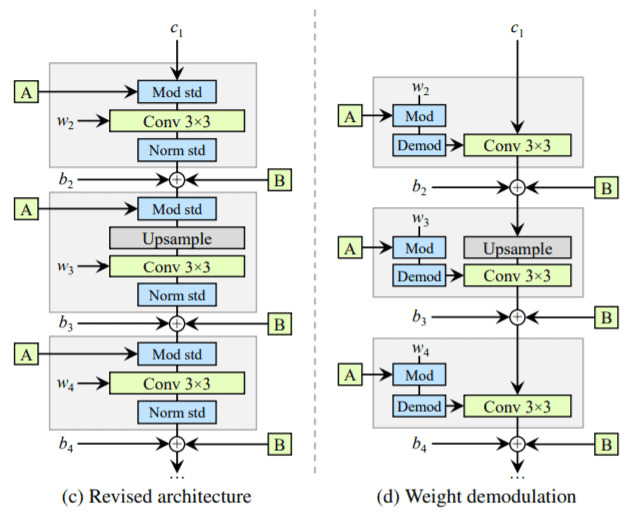
\includegraphics[width = 0.5\linewidth]{images/chapter3_img/styleblock.jpg}
        \caption{Διαμόρφωση και Αποδιαμόρφωση βαρών  στο αναθεωρημένο StyleBlock-StyleGan2, Πηγή \cite{karras2020analyzing}}
        \label{fig:styleblock2}
    \end{figure}

\par
    Τα δίκτυα που χρησιμοποιούνται σε αυτή την εργασία είναι μη συνελικτικά πλήρως συνδεδεμένα \enit{MLPs} μιας και η λογική της ανακατασκευής απαιτεί να μην γίνει μετασχηματισμός του χώρου του συνταγμένων με τρόπο που δεν λαμβάνει υπόψιν την ισομετρική ιδιότητα του χώρου.  Συνεπώς εργασίες όπως \cite{vaswani2023attention} (\enit{Attention is all you need}) δίνουν μια πιο γενική μορφή στο πως να βοηθήσουμε την έμφαση και την προσοχή που δίνει το δικτύου σε ορισμένα μόνο χαρακτηριστικά, ανεξαρτήτως αρχιτεκτονικής. Σε αυτή την λογική, βασίζονται πλέον όλα τα σύγχρονα μοντέλα που θέλουν να καταγράψουν το στυλ των δεδομένων. 